% Opcje klasy 'iithesis' opisane sa w komentarzach w pliku klasy. Za ich pomoca
% ustawia sie przede wszystkim jezyk i rodzaj (lic/inz/mgr) pracy, oraz czy na
% drugiej stronie pracy ma byc skladany wzor oswiadczenia o autorskim wykonaniu.
\documentclass[polish,inz,shortabstract, declaration]{iithesis}

\usepackage[utf8]{inputenc}

%%%%% DANE DO STRONY TYTUŁOWEJ
% Niezaleznie od jezyka pracy wybranego w opcjach klasy, tytul i streszczenie
% pracy nalezy podac zarowno w jezyku polskim, jak i angielskim.
% Pamietaj o madrym (zgodnym z logicznym rozbiorem zdania oraz estetyka) recznym
% zlamaniu wierszy w temacie pracy, zwlaszcza tego w jezyku pracy. Uzyj do tego
% polecenia \fmlinebreak.
\polishtitle    {Wykorzystanie sieci neuronowych do wykrywania zmian\fmlinebreak w obrazach medycznych}
\englishtitle   {English title}
\polishabstract {Celem projektu jest wykorzystanie modelu VAE do wykrywania zmian patologicznych w obrazach medycznych}
\englishabstract{\ldots}
% w pracach wielu autorow nazwiska mozna oddzielic poleceniem \and
\author         {Tomasz Nanowski}
% w przypadku kilku promotorow, lub koniecznosci podania ich afiliacji, linie
% w ponizszym poleceniu mozna zlamac poleceniem \fmlinebreak
\advisor        {dr Jan Chorowski}
%\date          {}                     % Data zlozenia pracy
% Dane do oswiadczenia o autorskim wykonaniu
\transcriptnum {279076}                     % Numer indeksu
\advisorgen    {dr. Jana Chorowskiego} % Nazwisko promotora w dopelniaczu
%%%%%

%%%%% WLASNE DODATKOWE PAKIETY
% 
\usepackage{graphicx,listings,amsmath,amsthm,amsfonts,tikz}
\usepackage[colorinlistoftodos]{todonotes}
%
%%%%% WŁASNE DEFINICJE I POLECENIA
%
% \theoremstyle{definition} \newtheorem{definition}{Definition}[chapter]
%\theoremstyle{remark} \newtheorem{remark}[definition]{Observation}
%\theoremstyle{plain} \newtheorem{theorem}[definition]{Theorem}
%\theoremstyle{plain} \newtheorem{lemma}[definition]{Lemma}
%\renewcommand \qedsymbol {\ensuremath{\square}}
% ...
\graphicspath{ {./images/} }
%%%%%

\begin{document}

%%%%% POCZĄTEK ZASADNICZEGO TEKSTU PRACY

\chapter{Introduction}



\chapter{Artificial neural networks}

Sztuczne sieci neuronowe mają obecnie bardzo mocno ugruntowaną pozycję szczególnie w dziedzinie problemów związanych z analizą i przetwarzaniem obrazów. Pomimo, iż nie jest to nowy pomysł, dopiero ostatni wzrost w wydajności komputerów pozwolił na ich praktyczne zastosowanie. Z matematycznego punktu widzenia są to sparametryzowane nieliniowe funkcje o pewnej ustalonej strukturze. Składają się z prostych elementów zwanych neuronami, a one natomiast są pogrupowane w warstwy. Połączenia między warstwami definiują przepływ danych. 'Nauka' sieci neuronowych polega na optymalizacji pewnej funkcji straty, czyli wyznaczeniu takich parametrów, żeby osiągnąć minimalny koszt. Do tego celu często korzysta się z metod opartych na SGD, a przy wybranej strukturze można w efektywny sposób zastosować algorytm propagacji wstecznej. W dalszej części pracy będę używał prostszej nazwy (neural nets). Przykładowa architektura sieci neuronowych jest zaprezentowana na wykresie ???.

\section{Autoencoders}

Jest to jeden z rodzajów sieci neuronowych, służący do znajdowania wydajnej reprezentacji danych, co jest przykładem nauki bez nadzoru. W autoencoder'ach mozna wyróżnić dwie części: encoder i decoder. Zadaniem encodera jest wyprodukowanie reprezentacji, natomiast decoder służy do odtworzenia z niej oryginalnej postaci. Zależy nam na tym, żeby wyjście było w jakimś sensie jak najbardziej podobne do wejścia. W przypadku obrazów jako funkcja straty często stosowane jest MSE. Przykładowy schemat na wykresie \ref{fig:autoenc}.

\begin{figure}[h]
    \centering
    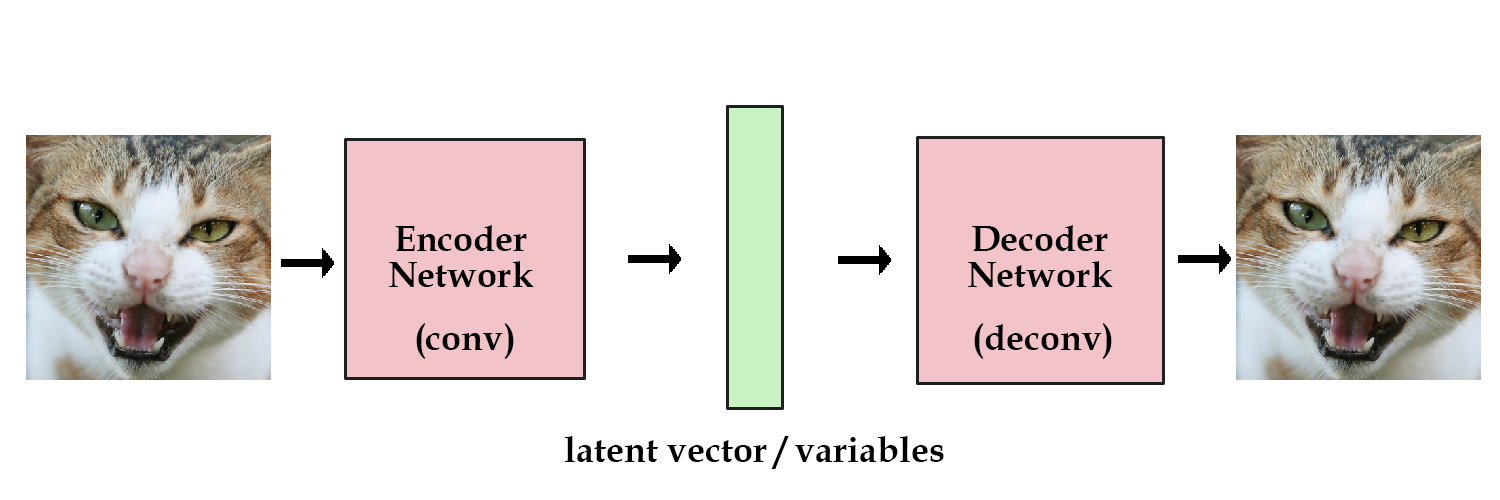
\includegraphics[width=1\textwidth]{autoenc}
    \caption{Architecture of autoencoder}
    \label{fig:autoenc}
\end{figure}

\section{VAE}

Variational autoencoders rezszerzają założenia o wprowadzenie modelowania rozkładu prawdopodobieństwa dla reprezentacji ukrytej. 

\section{Convolution VAE}

Jest to rozszerzenie poprzedniego modelu, w którym dodatkowo stosujemy warstwy splotowe. Szczególnie w przypadku obrazów pozwala to na zwiększenie rozmiaru danych wejściowych przez zmniejszenie ilości parametrów w stosunku do warstw fully-connected oraz wykryciu na wstępie jakiś prostych cech, przez co w reprezentacji mogą znajdowac się bardziej abstrakcyjne rzeczy. 

\section{Deep feature consistent variational auto-encoder}

Ta wersja zakłada użycie innej funkcji kosztu. MSE z samej definicji przyczynia się do uśredniania wartości pikseli przez co wyjściowy obraz nie jest wyraźny. W tym przypadku będziemy korzystać z zewnetrznej sieci splotowej wyuczonej do klasyfikacji obrazów. Będziemy teraz myśleć, że dwa obrazy są podobne, jeśli maja podobne wartości aktywacji w tej sieci. Takie podejście powinno nam dać ostrzejsze wyjście.

\chapter{MNIST experiments}

\section{MNIST}

Jest to zbiór pokategoryzowanych odręcznie napisanych cyfr. Wszystkie obrazki są czarno-białe, rozmiaru 28x28 i wycentrowane. Zbiór składa się z 60000 danych treningowych i 10000 testowych. Zbiór ten często wykorzystywany jest w celu ekperymentowania z modelem, jednak jest na tyle mało skomplikowany, że daje jedynie poglądowe informacje. Przykładowe obrazki \ref{fig:mnist}.

\begin{figure}[h]
    \centering
    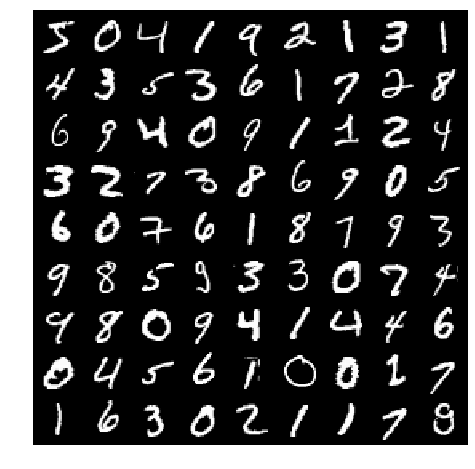
\includegraphics[width=0.5\textwidth]{mnist}
    \caption{Samples from MNIST dataset}
    \label{fig:mnist}
\end{figure}

\section{VAE}

Wyniki przy użuciu zwykłego VAE

\begin{figure}[h]
    \centering
    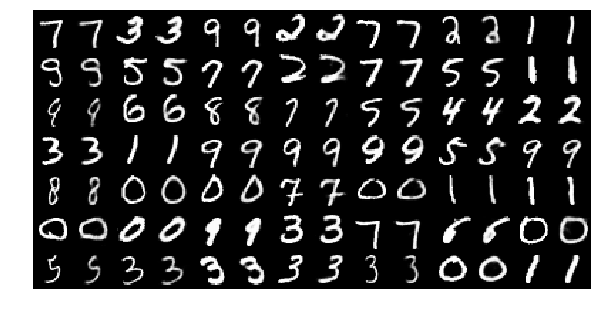
\includegraphics[width=1.0\textwidth]{mnist_recon}
    \caption{}
    \label{fig:mnist_recon}
\end{figure}

\begin{figure}[h]
    \centering
    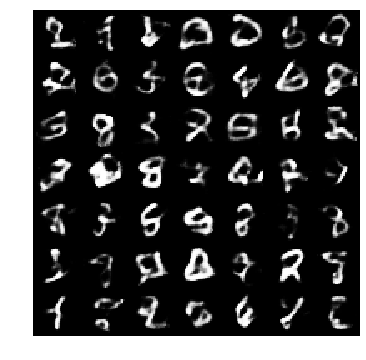
\includegraphics[width=0.6\textwidth]{images/mnist_gen.png}
    \caption{}
    \label{fig:mnist_gen}
\end{figure}

\section{Deep feature consistent variational auto-encoder}

Wyniki przy użyciu Deep feature consistent variational auto-encoder.

\chapter{Medical Dataset}

Dane pochodzą z Uniwersytetu ... z USA.

\section{Description}



\section{Preprocessing}

Opis preprocessingu

\section{Patches}

Wybór rozmiaru patchy i ekspeymenty z tym związane

\section{Normalizations}

\todo{Może LIME?}

\chapter{Experiments on medical dataset}

\section{VAE}

\section{C-VAE}

\chapter{Workflow}

\chapter{Summary}


%%%%% BIBLIOGRAFIA

%\begin{thebibliography}{1}
%\bibitem{example} \ldots
%\end{thebibliography}

\end{document}
